\chapter{Previous work}

The previous sections have established the context, and identified the primary areas of relevant literature. From biology, the main threads concern the origins of life, and the theory of evolution. Natural selection provides the primary mechanism for evolution in biology, although it is not the only process at work -- genetic drift and neutral theory provide a counterpoint. In artificial systems, researchers have used biological evolution as an inspiration, gradually over time diverging into a field with the beginnings of its own motivating theory, now only loosely connected with its origins in the natural world.

The research emphasis in artificial systems has more recently returned to a reappreciation of how biological evolution generates robust, novel, creative outcomes, unlike those seen in current artificial evolution. This has led to a renewed interest in understanding the principles behind biological evolution so that artificial systems can capture some of those admirable properties; the difference now is that the transference is sought at the level of concepts and principles rather than in the historical inspiration of specific biological elements and structures, many of which are contingent and perhaps even arbitrary; certainly complex.

This section now expands upon previous work that is directly relevant to our specific problem, the onset of evolution in artificial systems, in two areas:

\begin{itemize}
	\item General evolutionary models
	\item Specific work in artificial systems
\end{itemize}

\section{General evolutionary models}

There is now a body of literature where the goal is to abstract general principles of evolution from the specifics seen in particular fields.

In biology, population genetics describes the dynamics over time of genotype frequencies, and Waddington explored the requirements for open-ended ongoing evolution.
In theory of computation, Von Neumann machines provide the first detailed recipe for self-replicating machines.
Paixao2015 sought common principles between population genetics and evolutionary computation in an attempt to unify the two fields. Similarly MWUAs seek a deeper meaning to evolution, placing it as one of a family of closely related algorithms all based on multiplicative weights.

\subsection{Population Genetics}

\autocite{Paixao2015}:
		
		PG evolution described by dynamics of allele or genotype frequencies
	
		Lewontin 1964 equation for canonical evolutionary process - genotype
		frequencies, based on common ``genetic operator'' for rate of
		generating a genotype x from parents y and z (combines mutation,
		recombination etc)

		This and other models biologically focussed - where ``selection
		assumes a particular form''

		Another approach to PG quantitative genetics - phenotypic view of
		trait evolution. Useful in animal breeding. Doesn't address
		mechanism (genetics)

		Price equation - very general, useful for that reason in comparing
		models

\autocite{VonNeumann1966} as reviewed in \autocite{Taylor1999} (Lack of environmental emphasis)
Von Neumann's architecture for how ``complicated machines could evolve from simple machines''

\begin{enumerate}[label=\Alph*]
	\item A \emph{constructive} machine that takes a description and builds a new machine;
	\item A \emph{copying} machine to make a copy of a description, and 
	\item A \emph{control} machine to sequence the other two machines - first the copying machine, then constructive, then finally to link the new machine to its description.
\end{enumerate}

Von Neumann makes a fundamental distinction between a description of a machine and the machine itself; in biological terms, the architecture separates between genotype (description) and phenotype (the machine.) However, because some of the function of the three machines (A, B, C) are provided by the world there is a limit to how self-referential the system can be, and hence how much its function can evolve over time.

Taylor states ``I would suggest that the reproducing programs in Tierra and similar systems can also sensibly be analysed in terms of von Neumann's architecture.''

Just a few years later, 
\autocite{Waddington2008} as reviewed in \autocite{Taylor:1999sc}--Originally published in ``Towards a Theoretical Biology, Vol. 2'' in 1969

Also Genotype (G) and Phenotype (Q*) based, where Q* associated with
an environment (E from Ej)

For OEE need: Ej infinite numbered set, and sufficient Qs for Q*s
for all those Ejs

Q*s are part of Ej satisfies condition one {[}recursive?{]}

Second is an emergent one - ``it is not sufficient to create new
mutations which merely insert new parameters into existing
programmes; they must actually be able to rewrite the programme''
- key distinction between OEE and creative evolution

\autocite{Paixao2015}:

	attempt to unify evolutionary computation and population genetics -
	based on common conception of evolutionary process


	Any evolutionary process describes ``population undergoing changes
	over time based on some set of transformations''

	A transformation can be decomposed into a collection of (stochastic)
	operators. Operator can be described as a probability distribution of
	potential outcomes; and evolutionary process as a trajectory through a
	space of distributions.
	
	Process described both as a sequence of population transformations,
	and as distribution transformations

	
	Individuals described with both genotype and phenotype; gp mapping
	between them. Some operators act on genotype others on phenotype

	
	Various operators defined - for selection (uniform, proportional,
	tournament, truncation, cut, replace); variation (mutation) (uniform,
	single-point), variation (recombination) (one-point crossover, k-point
	crossover, uniform crossover, unbiased variation)

	Most models satisfy five given mathematical properties
		
	\begin{itemize}
		\item
		
		V1 - uniformity preserving - no change to distribution if uniformly
		distributed
		
		\item
		
		M1 - mutation acts on individuals
		
		\item
		
		M2 - mutation can generate whole search space ie an ergodic operator
		(defining characteristic of mutations)
		
		\item
		
		R1 - recombination preserves allele frequencies (in expectation)
		
		\item
		
		S1 - selection doesn't change individuals
		
	\end{itemize}

	Demonstrates how existing ``classical models in theoretical population
	genetics and in the theory of evolutionary computation'' can be mapped
	into this framework. Most of PG models can be represented
	(unsurprising as most variants of classical models that have been
	demonstrated in framework); some topic-specific EC models could not be
	- but not ones that have a relationship with PG and so of little
	interest to biologists. GP models omitted for reasons of balance
	between simplicity and inclusiveness
	
	Leaves MOEAs for later work

	``In an Estimation Distribution Algorithm (EDA), the algorithm tries
	to determine the distribution of the solution features, e.g.
	probability of having a 1-bit at a particular position, at the
	optimum. Some EDAs can be regarded abstractions of evolutionary
	processes: instead of generating new solutions through variation and
	then selecting from these, EDAs use a more direct approach to refine
	the underlying probability distribution. The perspective of updating a
	probability distribution is similar to the Wright--Fisher model.''
		
	\begin{itemize}
		\item
		
		Close similarity between simplest EDA (the Univariate Marginal
		Distribution Algorithm) and Linkage equilibrium models in population
		genetics as pointed out in Chastain2014 (``We demonstrate that in
		the regime of weak selection, the standard equations of population
		genetics describing natural selection in the presence of sex become
		identical to those of a repeated game between genes played according
		to multiplicative weight updates (MWUA), an algorithm known in
		computer science to be surprisingly powerful and versatile. MWUA
		maximizes a tradeoff between cumulative performance and entropy,
		which suggests a new view on the maintenance of diversity in
		evolution.'')
		
		\item
		
		AdaBoost is a form of MWUA
		(\href{https://www.cs.princeton.edu/~arora/pubs/MWsurvey.pdf}{\emph{https://www.cs.princeton.edu/\textasciitilde{}arora/pubs/MWsurvey.pdf}})
		
	\end{itemize}

\subsection{MWUA}

\autocite{Barton2014}

	Experts in MWUA equivalent to alleles in NS

	In selection, ``frequency of each type {[}allele{]} is simply
	multiplied by its relative fitness; which corresponds precisely to
	MWUA''
	

	MWUA ``maximizes the sum of two quantities: the expected total fitness
	of the chosen allele, summed over past generations, plus the entropy,
	which is a measure of the allelic diversity.''
	
	
	Fitness differences increase over time, and so population converges
	towards type with best performance; entropy term acts to slow down
	this convergence
	

	Problems
	
	
	\begin{itemize}
		\item
		
		because MWUA is deterministic, and some interesting problems e.g.,
		recombination as a mechanism for reintroducing gene combinations
		lost through drift in finite populations, are essentially
		stochastic, MWUA cannot address them
		
		\item
		
		Value of sex - MWUA applies equally to sexual and asexual
		populations so hard to gain insights as to role of sex
		
	\end{itemize}

\autocite{Chastain2014}:

	Assumes weak selection - from paper: differences in fitness between
	genotypes are small relative to the recombination rate and so
	evolution proceeds near linkage equilibrium - probability of
	occurrence of a certain genotype is the product of the probabilities
	of each of its alleles
	
	
	\begin{itemize}
		\item
		
		{[}Weak selection where two phenotypes have similar fitness, and so
		one only slightly preferred. Only relevant (claim elsewhere -
		wikipedia) that only relevant in Moran process (fixed population as
		births-deaths paired - no birth without a death) as in growing
		population both can proliferate and weak selection results in
		effectively no selection{]}
		
		\item
		
		{[}Also assumes sexual reproduction - ``in the presence of sexual
		reproduction'', and does not address mutation{]}
		
	\end{itemize}

	
	Shows that ``equations of population genetic dynamics are
	mathematically equivalent to positing that each locus selects a
	probability distribution on alleles according to a particular
	rule...known as the multiplicative weight updates algorithm (MWUA)''
	
	
	\begin{itemize}
		\item
		
		Uses Nagylaki's theorem for allele frequencies given weak selection
		in presence of sex
		
		\item
		
		NS is ``tantamount to each locus choosing at each generation its
		allele frequencies in the population so as to maximize the sum of
		the expected cumulative differential fitness over the alleles, plus
		the distribution's entropy.''
		
	\end{itemize}

	
	Hints that MWUA enhances entropy of alleles' distribution, so helping
	to maintain genetic diversity under NS - a ``tradeoff between
	increasing entropy and increasing (cumulative) fitness.''
	

\section{Elements of biological evolution}
	
\autocite{Hogeweg1998}

	``The simplest way of defining an evolutionary process is to define
	some set of predefined interactions between replicators and subject
	one (or a few) of the parameters of the system to mutations (selection
	automatically ensues from the dynamics of the system).''

	
	``\ldots{}the processes associated with the major transitions are an
	automatic consequence of mutation and selection, due to the generation
	of higher levels of selection due to spatial self-organization.''
	

		iff the interactions between the replicators are defined locally
		(meaning spatially) (from earlier work)
		

		because local interactions will form ``higher-level structures
		(e.g., spiral waves, turbulence, path like structures of different
		sizes) which constitute different levels of selection.''

		stress is on new levels of selection, rather than other elements of
		transitions

		
		But still ``they do not give us `novel' entities, as biotic
		evolution undoubtedly has''. Perhaps because lack one of the elements in Maynard-Smith:1995lw -
			``transition from limited inheritance to universal inheritance''
			

			Claim see other three in earlier work:
			
			\begin{itemize}
				\item
				
				Symbiogenesis - ``properties of local interacting, evolutionary
				systems ...embody a process reminiscent of `Symbiogenesis' in
				that self-sufficiency is (partly) given up in favor of the
				larger scale entities.''
				
				\item
				
				Conflicts among levels of selection - claims interactions
				between meso-scale and micro-scale entities are inherent (from
				observation of spiral wave experiments)
				
				\item
				
				Division of labour - different elements of spatial structure
				reproduce differently, hence germ-like and soma-like...
				
			\end{itemize}


	Necessary/essential for OEE - ability to redefine interactions,
	genetic representations, and fitness of the replicators

\autocite{Bourrat2015}


Difference between Evolution, Natural Selection and ENS


All from a biological reading; examples are regarding genes, traits,
phenotypes and drift and \ldots{}


And philosophical reading - epistemology regarding causality and
ability to reason - of earlier work e.g., `` So far this chapter has
shown that there is an alternative to the concept of fitness as a
propensity. I have argued for a concept of fitness as relational
properties between two or more individual entities forming a
population. I have shown, using causal graphs that distinguishing
between extrinsic and intrinsic-variable properties on the one hand
and intrinsic-invariable properties of entities on the other hand
could be the basis for distinguishing natural selection from
drift.`` {[}p65{]}
	

``The goal of the process perspective is to delimit what the minimal
requirements for a population to exhibit nothing but natural selection
(what I will call pure ENS) are. Thus, the goal here is to assess
whether the evolutionary change observed in a population with
imperfect transmission of traits across generations is compatible with
pure ENS. One way to carry out this evaluation is to consider a
population (albeit a highly idealised one) of entities in which all
the evolutionary forces except natural selection have been stripped
down: that is, one without mutation, migration and/or drift. In such a
case, any remaining evolutionary change in this population will be ENS
in its pure form. I call this class of populations, which is a
subclass of minimal Darwinian populations, pure Darwinian
populations.'' {[}p83{]}

``With this in mind, the strategy of endogenising can be understood
has explaining variables which have previously been taken for granted
in a model (such as reproduction and inheritance), by reference to
other, more fundamental variables present in the model.'' {[}p129{]}


Approach to demonstrate the imperfect inheritance is not compatible
with NS is to list three conditions for a population to evolve solely
by NS, and then show that at least one of those conditions is
incompatible with imperfect inheritance (as it happens, no production
of new variants) {[}p96{]} - argument by contradiction


Fundamental issue is that previous arguments proceed from biology
-\textgreater{} explanation by division, and then arguments over what
the divisions are. Bouratt attempts to bring clarity to the divisions
in order to come up with a consistent explanation for the biology. Our
goal is different - we're interested in the result not the explanation

Necessary steps for paradigmatic ENS p136 (slightly different from
conditions on p129 - wording, and conditions c and d swapped)
	
	
\begin{itemize}
	\item
	
	a ``New variation is introduced in the population over time''
	
	\item
	
	b ``The population is able to maintain its size or, if the size of
	the population is not limited, to increase (multiplication)''
	
	\item
	
	c ``Advantageous phenotypes are able to be transmitted during
	reproduction, making population-level changes against which new
	mutations can occur, possible.''
	
	\item
	
	d ``Reproduction is pervasive, therefore each entity in the
	population is in principle able to reproduce''
	
\end{itemize}

	
Modelling
	
\begin{itemize}
	\item
	
	Biased and unbiased \emph{inheritance}
	
	\begin{itemize}
		\item		
		Unbiased - trait is uncorrelated with parent. Implemented as
		random choice between lower and upper bound {[}p153{]}			
		\item	
		Biased - trait has correlation with parent, at some level. Some
		prediction of traits possible - parent can ``pass it on''. Not
		clear how the offspring traits are calculated though based on
		correlation {[}only description on p141 - later p173 expressly
		says this is not the `transmission bias` of the second term in the
		Price equation{]}. Looks like a narrowing of the gap between upper
		and lower bounds

	\end{itemize}
	\item
	
	Ability to \emph{procreate}	
	
	\begin{itemize}
		\item
		
		Persistors - unable to reproduce, selection only in ``weak'' sense
		of granite grains for hardness
		
		\item
		
		Procreators can reproduce but without inheritance of any property
		(including ability to procreate) except ``fact of coming into
		existence and membership of that class'' (class is class of
		parents defined by ``those properties that do not vary in the
		population''...{[}acknowledged as loose, but has benefit that no
		varying traits included{]}) p137. Procreator's offspring is
		persistors
		
	\end{itemize}
	\item
	
	Classes in models
	
	
	\begin{itemize}
		\item
		
		Minimal reproducers - indefinite procreation - where procreation
		can be transmitted from parent to offspring (with some low degree
		of fidelity)
		
		\item
		
		Unreliable reproducers (low bias for ability to procreate- ability
		to procreate randomly chosen between 0 and parent's ability),
		reliable reproducers (high bias - ability to procreate is same as
		parent's ability)
		
		\item
		
		Replicator - all traits (including procreation) can be inherited
		
	\end{itemize}
	\item
	
	All models assume property has occurred (so exogenous) and then
	investigates implications e.g., mutation or reproducer at
	onset\ldots{} {[}Models p149{]}
		
\end{itemize}

Models

\begin{itemize}
	\item
	
	Model 1
	
	
	\begin{itemize}
		\item
		
		5000 persistors, with random survival rate (viability) between
		0-0.99 (chance of surviving at each time step). Selection only.
		Essentially null hypothesis.
		
		\item
		
		All eventually die
		
		\item
		
		Viability reflects life-span; other events are proportional to
		life-span so procreators with long life-spans will produce more
		children, everything else being equal (note that standard
		meaning for fitness is viability*fertility)
		
	\end{itemize}
	\item
	
	Model 2
	
	
	\begin{itemize}
		\item
		
		4999 persistors and 1 procreator (survival rate, and fertility
		rate - offspring per unit time). Offspring traits uncorrelated
		with parent. Selection -\textgreater{} Reproduction
		-\textgreater{} Check-for-overcrowding (\emph{what is the
			ceiling on population size?})
		
		\item
		
		For procreator: Viability=0.99, fertility=10: all extinct a
		little later than in Model 1 (unsurprising)
		
	\end{itemize}
	\item
	
	Model 3
	
	
	\begin{itemize}
		\item
		
		Model 2 except single procreator replaced by single minimal
		reproducer - viability and fertility of offspring are unbiased,
		ability to procreate is unbiased also (so each offspring may or
		may not be able to procreate; ones that cannot are persistors).
		Viability selection is only form of selection in model
		
		\item
		
		Ability to procreate random between 0 and 0.20 (=probability
		offspring can procreate - looks as if same for each offspring,
		and same each generation - but unclear)
		
		\item
		
		Population size drops then increases to maximum size; about 10\%
		of minimal reproducers
		
		\item
		
		Proportion of high fitness (high viability=0.99) entities
		doesn't increase beyond about 0.05, so \emph{no cumulative
			adaptation}
		
		\item
		
		\emph{Surely also dependent on initial conditions - low rate of
			procreation will lead to extinction, high rate to proportion
			related to rate - calculable?}
		
	\end{itemize}
	\item
	
	Model 4
	
	
	\begin{itemize}
		\item
		
		Model 3 + (perfect) biased inheritance of viability (survival
		rate)
		
		\item
		
		Proportion of high fitness entities rapidly increases to near
		1.0 (near as some random decreases) - \emph{cumulative
			adaptation?}
		
		
		\begin{itemize}
			\item
			
			\emph{Mechanism is that high viability entities live longer
				and so produce more offspring/low viability die sooner and so
				produce less - fertility random, but viability heritable}
			
		\end{itemize}
		\item
		
		\emph{Why have persistors in initial population? Just die off -
			affecting proportions\ldots{}}
		
		\item
		
		\emph{Essentially just says that inheritance of viability +
			selection on viability =\textgreater{} adaptation towards high
			viability}
		
	\end{itemize}
	\item
	
	Model 5 - variable ability to procreate
	
	
	\begin{itemize}
		\item
		
		Model 3 + mutation stage
		(mutation-\textgreater{}selection-\textgreater{}reproduction-\textgreater{}check-for-overcrowding)
		
		\item
		
		At each mutation stage, 0.01 (also stated as 10\^{}-3...) rate
		for increase/decrease of ability to transmit ability to
		procreate (max 0.20 - reproducers), and degree of bias (that is,
		relationship to parent's ability) in ability to procreate (from
		unbiased to biased)
		
		
		\begin{itemize}
			\item
			
			in a sense, ability to procreate is a relationship between
			siblings (low ability of parent means low proportion of
			siblings can procreate, high ability means high proportion of
			siblings)
			
			\item
			
			while bias is the relationship between parent and offspring -
			low bias means offspring's ability is only weakly correlated
			with parents ability.
			
		\end{itemize}
		\item
		
		Viability (fitness) random 0-0.99; Ability to Procreate =
		initial random between 0 and 0.2, change +/- 0.01 equal
		probability; Bias initially 0, change +/- 0.01: max for both is
		1.0
		
		
		\begin{itemize}
			\item
			
			Both \emph{increase} over time in population -\textgreater{}
			1.0 - \emph{why? why does model not result in some infidelity
				or source of variation? }
			
			\item
			
			Asymmetry in direction of change of inheritance of ability to
			procreate - reductions lead to extinction of that line,
			increases lead to increased population\ldots{}
			
		\end{itemize}
		\item
		
		Conclusion: initial population of unreliable reproducers (low
		proportion of procreating offspring, no bias) results in
		reliable reproducers - all offspring are procreators
		
	\end{itemize}
	\item
	
	Model 6
	
	
	\begin{itemize}
		\item
		
		Population of reproducers with perfect bias in ability and
		fidelity of reproduction (end state of Model 5) + mutation on
		viability, and fidelity of transmittal of viability to offspring
		
		\item
		
		5000 individuals, viabilities random between 0 and 0.99;
		fertility between 0 and 10.
			\item
			
			Fidelity of viability \emph{increases} to 1.0

	\end{itemize}
\end{itemize}
		
Results
		
		
\begin{itemize}
	\item
	
	Minimal reproduction (not procreation) introduced through a)
	allows b), requiring only unbiased inheritance
	
	\item
	
	Unbiased inheritance of procreation and traits insufficient for c)
	
	\item
	
	Biased inheritance of trait (e.g., viability) satisfies c)
	(``Minimally-reproductive cumulative ENS''), but with unbiased
	inheritance of procreation doesn't meet d)
	
	\item
	
	Biased inheritance of trait + procreation meets c) and d)
	
\end{itemize}
		
	
Issues
	
	
\begin{itemize}
	\item From models with particular assumptions -\textgreater{} run
		(not known how many runs - other than references to ``typical run'')
		-\textgreater{} analyse output.
	
	\item Not known how sensitive models are to parameters (e.g,
		survival rates, fertility rates\ldots{}or inheritance of viability
		rate - in Model 4 rate is 1=perfect inheritance. Other arbitrary
		features: check for overcrowding stage in Model 2 onwards,
		introduced without justification p141)
	
	\item Why do factors in Models 4/5/6 increase to 1.0? What happens
		if start at 1.0? Would they drop? Results seem inconsistent with a
		hypothesis of useful variation\ldots{}
	
	\item Heredity and fitness (viability) are treated as independent
		traits. But mechanism for heredity is the thing that copies the
		information that generates an offspring's traits - so not
		independent. This might explain trait values trending to 1.0 rather
		than a lesser value consistent with a hypothesis of heredity as
		source of variation
	
\end{itemize}
	
\autocite{Watson2010}:

	Adaptation in biology appears to precede Natural Selection, so adaptation is possible without NS \autocite{Watson2010}

	Fundamental open question - mechanisms for adaptation
	
	Explored through variety of different projects, self-organized
	adaptive systems without NS - ``We present an abstract model and
	simulation of this process and discuss how it relates to a number of
	different domains: the evolution of evolvability in gene regulation
	networks {[}12{]}, the evolution of new units of selection {[}10{]}
	via symbiosis {[}15{]} and 'social niche construction' {[}8,9{]},
	games on adaptive networks {[}2{]}, distributed optimisation in
	multi-agent complex adaptive systems {[}13,14{]} and multi-scale
	optimisation algorithms {[}6,7{]}.``


\autocite{Saunders1994} Evolution without Natural Selection (DaisyWorld):

	Lack of proof that NS was mechanism of natural evolution {[}still
	discussion e.g., Masatoshi Nei stressing mutation as driver;
	acceptance e.g, Mayr, that Darwin couldn't prove NS as mechanism for
	adaptation{]}

	
	Lovelock proposed Daisyworld as alternative explanation (rather than
	selection) for regulation as seen in Gaia hypothesis, and in organisms
	

	Two feedback loops lead to regulation, ``As a result, regulation, one
	of the most fundamental and necessary properties of organisms, appears
	without being selected for. What is more, it appears as a property not
	of the daisies, on which natural selection may have acted, but of the
	planet, on which, as Dawkins rightly points out, it could not.''
	
	
	The fundamental insight in Daisyworld is that individuals modify environments: the daisies adapt planet (temperature for maximum growth) to suit themselves, rather than adapting themselves to the planet.
	
	Little benefit to adaptation by daisies to planet. In fact, ``the
	ability to withstand a greater variability is not the result of
	Darwinian adaptation. On the contrary, it exists because of the
	absence of Darwinian adaptation.''

	``What is especially interesting for biology is that the problems
	arise when we try to optimize simultaneously two connected features of
	a structure. They will therefore not be revealed by a research
	strategy which seeks to account for organisms by decomposing them into
	individual traits which, so it is assumed, are acted on separately by
	natural selection.'' -- an argument for a holistic rather than reductionist view.

\autocite{Maley1999}

	``we would like the evolutionary system, like life, to continue to
	produce individuals of increasing complexity and diversity.'' -
	although note, following McShea, that much of life is single-celled
	and hasn't become much more complex in billions of years.

	
	Focus on diversity (to make progress)
	
	
	Some suggestions previously that diversity is bounded (at minimum, by
	number of molecules available for biosphere, also by energy and
	minimal populations and probably other things), and plateaus
	(punctuated equilibrium). Indicates two time constants
	
	
	\begin{itemize}
		\item
		
		fast - expansion to use available resources
		
		\item
		
		slow - innovations to open new adaptive space
		
	\end{itemize}

	
	Urmodel1 - neutral landscape, mutation, early stop before all niches
	filled (to prevent edge effects)
	
	\begin{itemize}
		\item
		
		32-bit genotype - mutation flips one-bit
		
		\item
		
		Get unbounded diversity, but no selection or heritable effect on
		fitness
		
	\end{itemize}
	
	Posits that need selection : ``Requirement 2 An open-ended
	evolutionary system must embody selection'' - because ``fails to meet
	one of the basic criteria of natural selection: the heritable
	variation has no effect on fertility'' {[}ignoring use of fertility as
	a fitness-analogue{]}, and from Bedau ``Requirement 3 ...continuing
	(`positive') new adaptive activity'' {[}ignore neutral theory, and
	accepts Bedau - perhaps to allow use of Anew as measure?{]}
	

	Urmodel2 - natural selection: mutation, ``dissimilarity'' for
	competitive advantage (justified by biological example of niche
	overlap theory (Levins, 1968)) - no increase in Anew
	

	Urmodel3 - selective sweep (hypothesis): parasites (mutations) and
	hosts (fixed genotypes). Fitness on degree of match between parasite
	and host bit patterns.
	
	
	\begin{itemize}
		\item
		
		Claim shows unbounded activity - ``the first known artificial
		evolutionary system demonstrating unbounded evolutionary activity''
		
		\item
		
		Restricted by 32-bit genomes, no death
		
		\item
		
		But probably not a unique or even significant result - ``The only
		trick is to defer the point when the model hits its true asymptotic
		behaviour for long enough that the growth dynamics of the model are
		themselves asymptotic in some sense''
		
	\end{itemize}

	
	Urmodel4 - ``the most important aspect of an organism's environment
	are the other organisms with which it interacts'' - add coevolution to
	Urmodel3 by letting hosts mutate
	
	Two ``distasteful aspects of Urmodel3'' leading to belief that metrics
	aren't right
	
	
	\begin{itemize}
		\item
		
		niches are imposed from outside, not endogenous - this becomes
		Requirement 4
		
		\item
		
		no surprise - claim is because not complex - ``A puddle of inert,
		multicoloured and diverse algae would not be nearly so inspirational
		as the rain forest.'' Again, a biological metaphor.
		
	\end{itemize}


\autocite{Watson2015}:

	Darwinian machine is fundamentally self-referential - products of
	evolution affect process of evolution - lots of examples
	
	\begin{itemize}
		\item
		
		Major transitions in evolution not possible without
		self-referentiality - unit of evolution must change between levels
		e.g., from molecules to cells. This was/is accomplished by changing
		the way that individuals interact, from competition to cooperation
		(fitness change) to form the next level. How does selection at one
		level get suppressed, and introduced at the next?
		
		\item
		
		Maynard-Smith/Szathmary
		
		\item
		
		Independent replication before transition, must replicate as part of
		a larger whole afterwards
		
		\item
		
		Fundamental for complexity - complexity associated with levels
		
		\item
		
		Draws analogy with Hinton 2008 Deep Learning
		
		\item
		
		At one level, supervised learning improving adaptation; at next
		higher, unsupervised improving robustness
		
		\item
		
		Modes of inheritance (for groups)
		
		
		\begin{itemize}
			\item
			
			``migrant pools'' - particles disperse horizontally and reform
			into new pools - type 1 group selection - no group inheritance
			
			\item
			
			Group fissioning - vertical inheritance - group inheritance
			(differences are heritable) - type 2
			
		\end{itemize}
	\end{itemize}


\autocite{Griesemer2001}
	
	examination of difference between Lewontin and Maynard Smith's views
	of units of selection/evolution

	Maynard-Smith
	\begin{itemize}
		\item
		
		``if there is a population of entities with multiplication,
		variation and heredity, and if some of the variations alter the
		probability of multiplying, then the population will evolve.
		Further, it will evolve so that the entities come to have
		adaptations....''
		
		\item
		
		M,V,H necessary for units of evolution. F sufficient for evolution
		of adaptations (with proviso in text)
		
		\item
		
		Units of evolution that have F are units of selection. Units of
		selection though do not imply units of evolution as not all MVHF
		necessary.
		
	\end{itemize}
	
	Lewontin
	\begin{itemize}
		\item
		
		phentotypic variation, differential fitness, fitness is heritable
		(by generalizing from Darwin 1859 p61) ``Owing to this struggle for
		life...Natural Selection\ldots{}''
		
		\item
		
		``These principles mention quantities that describe quantitative
		roles of causal capacities (Woodward, 1993)''
		
	\end{itemize}
	
	Darwin's concept of inheritance in 1859 p61 includes heritability (a
	capacity) and inheritance (a process carrying the capacity)
	
	\begin{itemize}
		\item	
		Lewontin stresses first, assuming second, and Maynard Smith's
		multiplication is about the second; his heredity is both.
		
	\end{itemize}

\section{Evolvability of Evolvability}

Pigliucci2008 - ``Is evolvability evolvable?''

\section{Approach and methods}\label{approach}

\begin{itemize}
	\item
	Want to remove extraneous factors as factors introduce complications
	\item
	Identification of necessary conditions vs contingent factors
	\item
	Ideally minimal choices to be made or parameters to be chosen
\end{itemize}

Untangle the general from the biological in previous work. Emergent, self-improving, actionist (similar to Brooks in AI)

Much previous work aimed at understanding biology--assumes that domain.

\begin{figure}
	\begin{center}
		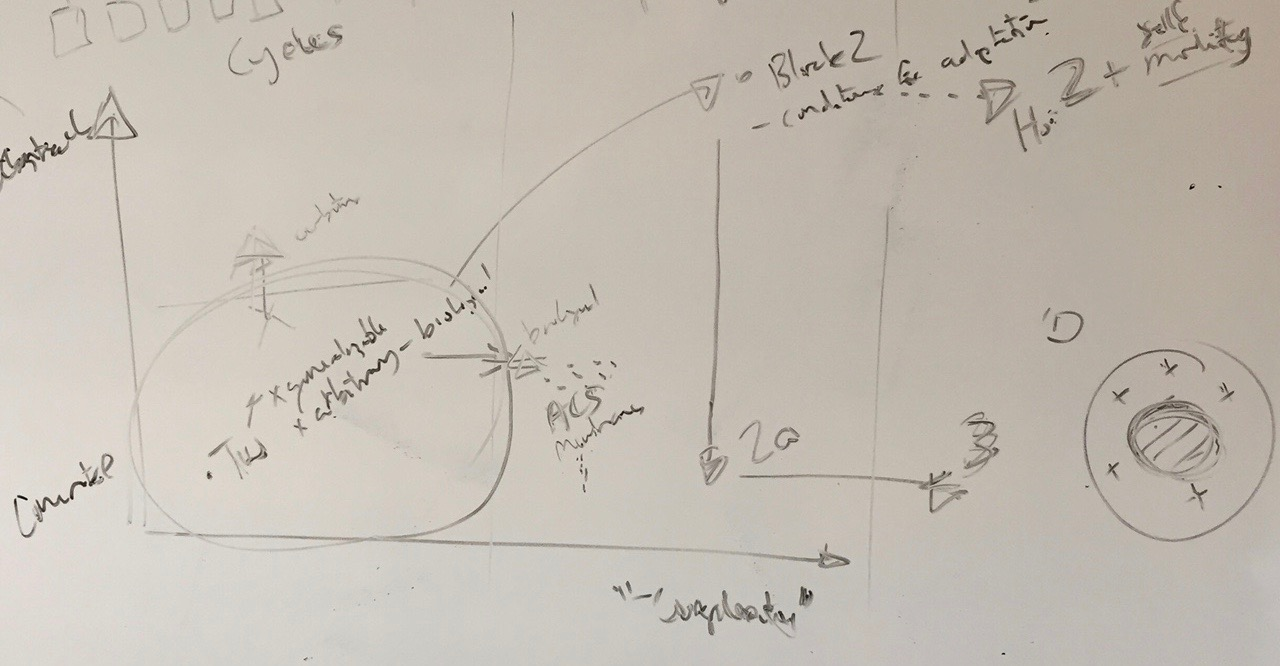
\includegraphics[width=\linewidth]{figures/approach}
	\end{center}
\end{figure}

\TODO{rewrite, properly mark quotations + references!}

The field of artificial life is synonymous with simulation
\autocite[chap.2]{Aicardi2010}. In other forms of science however
practitioners make use of a number of tools, including experiments,
mathematical models, thought experiments, and simulations.
Each method is well suited to some types of
questions, and inappropriate for others. Is the use of simulation
justified for our proposed investigation?

Simulations are becoming central to some disciplines in natural history.
Ecology--\glspl{abm} or \glspl{ibm} (reviewed in
\autocite{DeAngelis2005}; also see
\autocite{Grimm:2006fk,Grimm:2005wd,Grimm:1999kf,Hogeweg:1990jz}).
\glspl{ibm} in Microbiolgy are seen as very close to Alife \autocite{Grimm:2009th}.

The value of simulation over experiments for
\gls{ibm} study lies in a reduction in costs; the difficulties in
cultivation of microbial populations (99\% of known species yet to be
cultivated), and significantly, that they form \quote{complex systems only
	poorly explained by reduction.}{\autocite{Ferrer:2008hv}} Emergence and
dynamic behaviours are important, and yet they are hard to capture with
mathematical models.

Types of investigation

\subsection{Thought experiments}\label{thought-experiments}

non-empirical, clarification, contradictions/dissonance, fast, cheap.

\subsection{Models}\label{models}

\quote{
	It is seldom the case in biology that a model is derived deductively
	from a more fundamental quantitative theory, with the possible exception
	of population genetics which has its foundations in evolutionary
	theory.}{\autocite{Krakauer2011}}

Models can be ``useful stop-gaps'' towards a theory, by providing a
testable body of data for experiments and predictions
\autocite{Krakauer2011}, and may be constructed either bottom-up (such
as in ABM) or top-down, by the application of constraints
\autocite{Krakauer2011}. Many types in \eg ecology--eleven according to
\autocite{Jorgensen2008}--of which fall into two main groups

Mathematical models: complexity, need for abstraction/assumptions
(\eg Fisher's famous equation describing the changes in allele
distribution under selection assumes independent genes--extending this
to realistic cases remains an open problem \autocite{Schuster2011}),
difficulty in handling dynamism/emergence. Cheap, fast. Non-empirical.

Simulations: bottom-up approaches, holistic, variability so diversity
closer to real systems, adaptive behaviour/changing
\autocite{Ferrer:2008hv}. Non-empirical data.

\subsection{Experiments}\label{experiments}

reductionism, conflation (difficulty in removing other factors e.g.,
Heinemann), expense, time (generations). Source of empirical data.

\quote{
	Although this may seem a paradox, all exact science is dominated by the
	idea of approximation.}{The Scientific Outlook, Bertrand Russell}

\subsection{Benefits}\label{benefits}

Unique ability to explore subject = unique object of enquiry e.g., study
of emergence, complex, self-organizing subjects. Biology stands alone in
the importance of emergence \autocite{Bersini:2006ve}, and the
interconnection of levels of analysis, \eg behaviour can influence gene
expression, and genes can affect behaviour \autocite{Krakauer2011}. As
summarized by \autocite{Krakauer2011}, when asking how much of biology
can be predicted bottom-up from the application of basic physical and
chemical laws--``This question is simple to answer: effectively zero.''

Unique method of enquiry, that is, properties that improve on existing
techniques, e.g., by relaxing assumptions

\subsection{The epistemological nature of simulations}\label{the-epistemological-nature-of-simulations}

Simulations seem to fall somewhere in between thought experiments or
abstract models, and experiments. They are also relatively novel; common
use has only come with increased access to digital computers.
Consequently the nature of simulation--what can be claimed as a result
of simulation, and what role may be played legitimately by simulation in
scientific discovery--is a hot topic for philosophers of science. As
might not be unexpected, there are two opposing positions taken, plus a
synthesis that claims the middle ground.

\newthought{Simulations are just calculators}\label{simulations-are-just-calculators}

a computational means to solve analytically intractable equations
\autocite[31]{Winsberg2010}, producing nothing new (just consequences
of what is ``fed in''\autocite{DiPaolo2000}), nothing empirical.

\quote{A simulation is ultimately
	only a high-speed generator of the consequences that some theory assigns
	various antecedent conditions.}{\autocite{Eldridge}, quoting from Dennett 1979 p192}

If a model, then might take many forms--analogy, model, pure exploration \autocite{Webb2009}.

Models are \quote{a purposeful representation. A model needs to have a
	purpose because otherwise there would be no way to decide what to
	include in it. A model's purpose is a filter: the model should not
	include anything not believed essential for explaining the phenomenon
	of interest}{\autocite{Grimm:2009th}}

\autocite{MaynardSmith1974} distinguishes between
``practical'' descriptions of ecological systems, or ``simulations'', and
theoretical ones: ``models''.

Simulations are aimed at answering specific questions, or analysing
particular scenarios. The more accurate the simulation however, and
hence the more valuable the results, the harder it is to generalize to
other cases. It is hard to understand the behaviour of complicated
simulations, and the causes of particular behaviours of interest may be
unclear if there are many variables in play.

Instead, \autocite{MaynardSmith1974} prefers the use of simple models, designed
to illuminate the ``causes of differences of behaviour between different
species or systems'' rather than ``assertions which are true of all
systems or of all species.''

Hughes 1999 would argue that simulations have genuinely ``mimetic''
character, particularly ones that present results graphically as
real-world systems do, that goes beyond plain number-crunching. They use
a variety of methods beyond calculation (such as graphics) to draw
inferences from data. They also incorporate approximations and creative
choices to make the problem tractable, which introduces need for
justification. Simulations need interpretation and justification--they
are not self-contained, their own justifications
\autocite[31]{Winsberg2010}

\newthought{Simulations are themselves an instance of the
	thing}\label{simulations-are-themselves-an-instance-of-the-thing}

That is, the thing is not a shadow but the object. The Animats are
actually alive, and therefore instances of biology.
\footnote{And this way leads us to the claims of Strong Alife--the simulation is actually alive.}
The simulation is a stand-in for the real world, and you can perform
experiments on it as would any other system
\autocite[31]{Winsberg2010}. As \autocite{Adami2002} says, describing
Avida,

\quote{
	These organisms, because they are defined by the sequence of
	instructions that constitute their genome, are not simulated. They are
	physically present in the computer's memory and live there. The world to
	which these creatures adapt, on the other hand, is
	simulated\ldots}{\autocite{Adami2002}}

They certainly have elements of uncertainty and error, like experiments.

TODO Paul Humphreys 1994 says Monte Carlo simulations are experiments; Von
Neumann ``replace a computation from an unquestioned theory by direct
measurement'' (quoted in TODO [28]{Winkler et al 1987}).

Norton and Suppe 2001 argue that they are experiments, when proper conditions met:
``Empirical
data about real phenomena are produced under conditions of experimental
control'', although ``lacking other data, we can never evaluate the
information that these experiments provide'' Hughes 1999 p.142 so no inherent epistemological force to his
argument. Validity solely depends on validation.

\newthought{A third-way, neither experimental or theoretical}\label{a-third-way-neither-experimental-or-theoretical}

\autocite[31]{Winsberg2010} or an Opaque Thought Experiment"
\autocite{DiPaolo2000}. A common view, among others Dowling 1999, 264:
simulation is like theory as about ``manipulating equations'' and
``developing ideas'' but like experiments as ``fiddling with machines'',
``trying ideas out'', ``watching to see what happens.'' Simulation is a
form of Kuhn's theory articulation or ``model building''--making
principles apply to local, concrete systems in the real world. In this
view, \quote{Simulation is a process of knowledge creation}{\autocite[6]{Winsberg2010}}

\subsection{The legitimate role of simulation in scientific
	enquiry}\label{the-legitimate-role-of-simulation-in-scientific-enquiry}

Following this third way, simulations might be seen as a source of new
hypotheses \autocite{Eldridge}. The fundamental question remains
however: what is the exact relationship between world and simulation? If
the simulation exhibits an analogous behaviour, under a set of
assumptions, to the real world, then we can contend that there exist
similar mechanisms in the real world to the assumptions in our model.
TODO Noble 1997, quoted in \autocite{Eldridge}). The example given by
\autocite{Eldridge} is Boids \autocite{Reynolds1987} where flocking behaviour in
birds is very similar to that that results from a set of three simple
rules in a simulation.

However, \autocite{Eldridge} identifies three problems with this
approach: first, logically, similarity does not require congruence
\autocite{Weitzenfeld1984}, second, how is the degree of similarity to
be assessed, and third, the impossibility of proving that a simulation
is an accurate model of a theory. That is, where does attribution lie?
Is the result a result of the underlying theory or a quirk of the
implementation? There may be no way of resolving this absolutely as it
may not even be possible to distinguish between the two
\autocite{DiPaolo2000}--we cannot prove correctness through testing.

TODO On the other hand, Taylor (1989) in \autocite{Webb2009}, argues for
``pure exploration'' or ``exploratory tools'' that do not need
justification, and that may be used to generate ``new questions to ask,
new terms to employ, or different models to construct'' (Taylor 1989,
p122). But in this case you might reasonably argue that any insights are
``insights about a mathematical system'' not necessarily insights into
the real-world (123–124 Taylor 1989).

In practice then, any form of model claiming a significance beyond its
own self must show a correspondence with the thing it claims to be
modelling.

\quote{However, existence proofs clearly do require comparisons
	between model results and empirical data. One cannot evaluate the claim
	that phenomenon X requires condition Y unless one can show that
	phenomenon X is actually produced (with or without Y). And the claim or
	proof will be stronger or weaker depending on how well the simulated X
	matches the real X; for example, demonstrating successful behaviour in
	the same physical situation as the animal.}{\autocite[278]{Webb2009}}
The strength of our belief depends on the degree of similarity.

